\documentclass[12pt, letterpaper]{article}
\usepackage[a4paper, total={6in, 8in}]{geometry}
\usepackage[utf8]{inputenc}
\usepackage{multirow}
\usepackage{graphicx}
\usepackage[table]{xcolor}

\title{Compte Rendu LO21 \#1}
\author{Philippe Lefebvre, Clea Bordeau, Thomas Habert, Eugène Valty}
\date{Novembre 2021}

\begin{document}

\maketitle

\renewcommand{\contentsname}{Sommaire}
\tableofcontents

\section{Introduction}
Ce premier compte rendu contient un début d'architecture pour le projet, décrivant les différentes classes et leurs interactions.\\
Comme demandé, une liste des différentes tâches ainsi que leur importance est aussi fournie.
\section{Architecture}
\subsection{Introduction}
Vous trouverez ci dessous un \textbf{début} d'architecture; plusieurs notions jugées très importantes pour le sujet n'ont pour l'instant qu'été seulement effleuré en cours \textit{(Hérédité, classe virtuelle, classe générique,...)}. L'architecture est donc voué à être modifiée dans le temps, mais à été réfléchie de façon à ce que chaque modification n'impacte qu'elle même en utilisant le principe d'\textbf{encapsulation}.\\
Les méthodes ne sont pas très exhaustives, mais seront précisés au fur et à mesures.
\subsection{UML}
\begin{figure}[h]
\centering
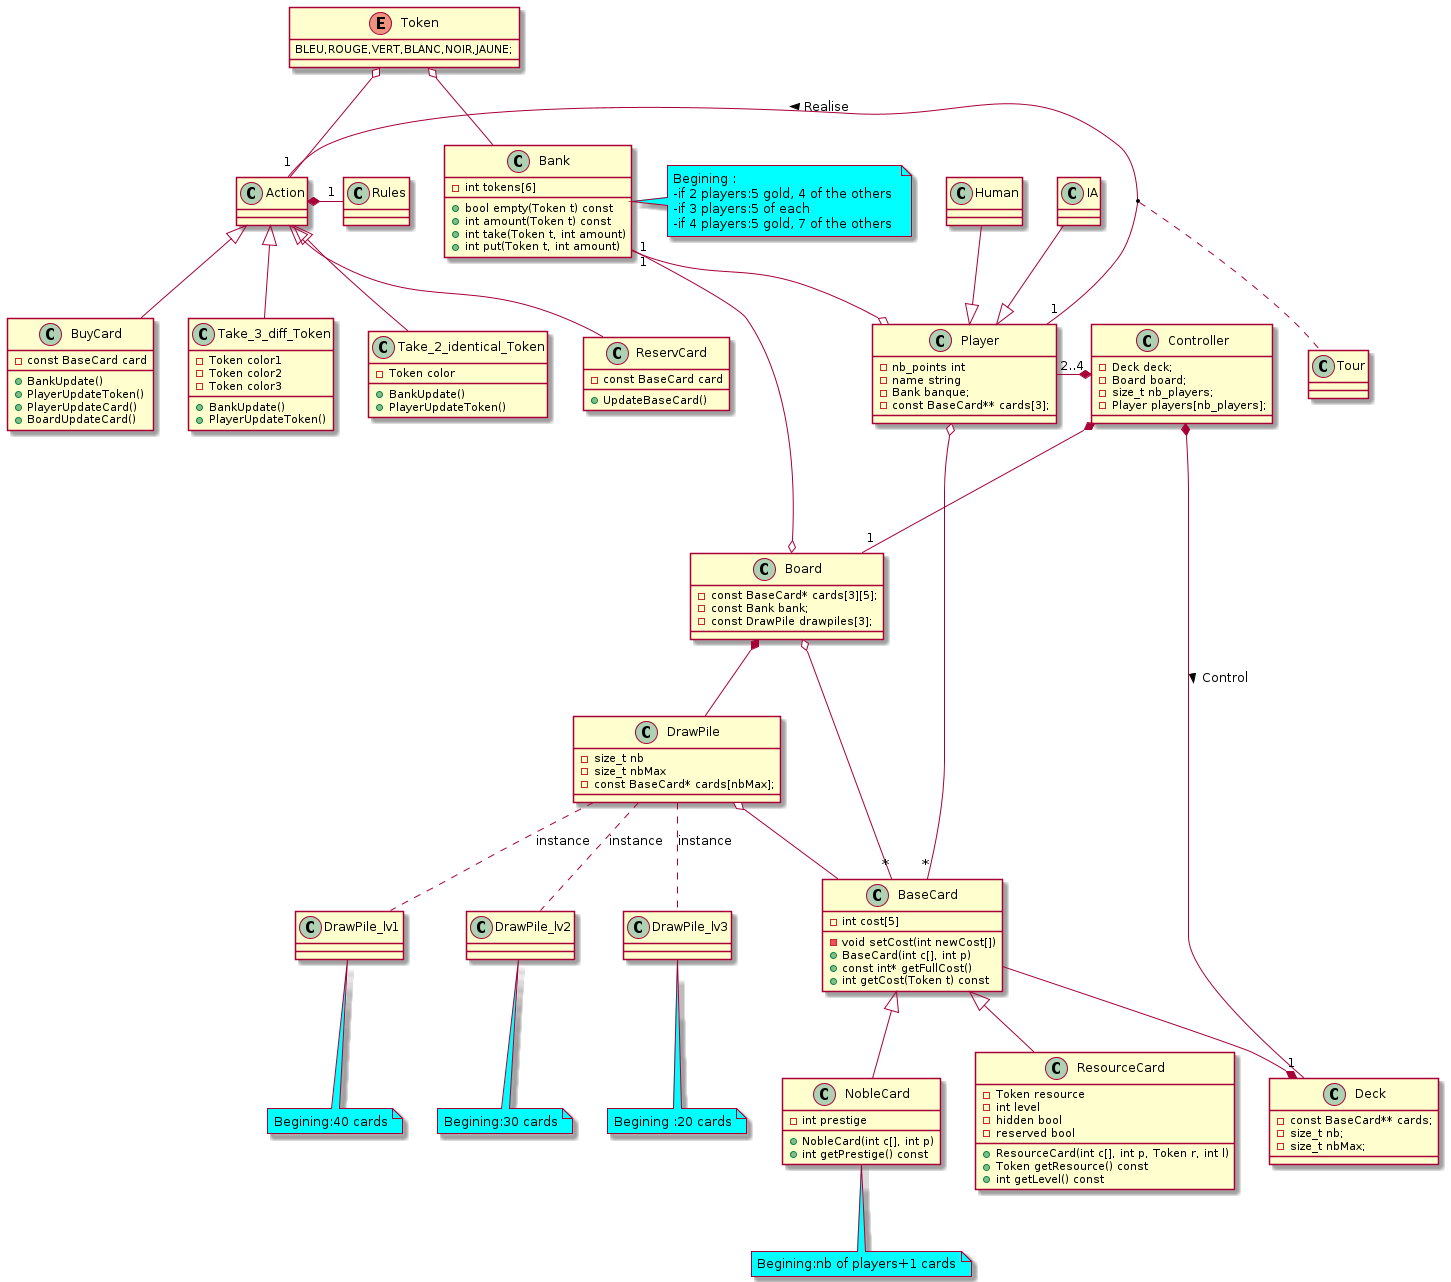
\includegraphics[width=\textwidth]{uml.png}
\caption{UML de l'architecture de base}
\end{figure}
\section{Tâches}
\subsection{Introduction}
La liste des tâches inclue essentiellement la construction de l'architecture de base. Il est évident que d'autres tâches \textit{(sur des fonctions spécifiques, des implémentations précises, ...)} viendront s'ajouter au fur et à mesure. On remarquera aussi que les tâches concernant la vue ne sont pas inclues; elles viendront s'ajouter lorsque le modèle sera fonctionnel.
\subsection{Liste des tâches}
\begin{center}
\begin{tabular}{ |c||c||c|p{5cm}| }
\hline
\multicolumn{4}{|c|}{Tâches} \\
\hline
Nom de la tâche & Numéro & Priorité & Prérequis\\
\hline
\hline
Ecrire la classe Token & 1 & \cellcolor[HTML]{ee7d7d} Indispensable & Aucun\\
\hline
Ecrire la classe BaseCard (générique) & 2 & \cellcolor[HTML]{ee7d7d} Indispensable & Aucun\\
\hline
Ecrire la classe NobleCard & 3 & \cellcolor[HTML]{eeda7d} Important & classe Cartes\\
\hline
Ecrire la classe ResourceCard & 4 & \cellcolor[HTML]{eeda7d} Important & classe Cartes\\
\hline
Ecrire la classe DrawPile (générique) & 5 & \cellcolor[HTML]{eeda7d} Important & Aucun\\
\hline
Ecrire la classe Deck &  6 & \cellcolor[HTML]{ee7d7d} Indispensable & classe Carte, classe Pioche\\
\hline
Ecrire la classe Bank & 7 & \cellcolor[HTML]{ee7d7d} Indispensable & classe Jeton\\
\hline
Ecrire la classe Board & 8 & \cellcolor[HTML]{ee7d7d} Indispensable & classe Carte, classe Pioche, classe Banque\\
\hline
Ecrire la classe Player (générique) & 9 & \cellcolor[HTML]{ee7d7d} Indispensable & classe Carte, classe Jeton\\
\hline
Ecrire la classe Player Human & 10 & \cellcolor[HTML]{eeda7d} Important & classe Joueur\\
\hline
Ecrire la classe Player AI & 11 & \cellcolor[HTML]{a5ee7d} Utile & classe Joueur\\
\hline
Ecrire la classe Action & 12 & \cellcolor[HTML]{eeda7d} Important & Aucun\\
\hline
Ecrire la classe Rules & 13 & \cellcolor[HTML]{ee7d7d} Indispensable & classe Action\\
\hline
Ecrire la classe Controller & 14 & \cellcolor[HTML]{ee7d7d} Indispensable & toutes les classes\\
\hline
Réaliser l'UML et l'architecture & 15 & \cellcolor[HTML]{ee7d7d} Indispensable & Aucun\\
\hline
\end{tabular}
\end{center}
\subsection{Informations sur les tâches}
\begin{center}
\begin{tabular}{ |c||c||c|c|c| }
\hline
\multicolumn{5}{|c|}{Tâches} \\
\hline
Nom de la tâche & Numéro & Assigné à & Durée estimée & Avancement\\
\hline
\hline
Ecrire l'enum Token & 1 & Philippe & -1h & 0\%\\
\hline
Ecrire la classe BaseCard (générique) & 2 & & 2h & 0\%\\
Ecrire la classe NobleCard & 3 & Philippe & 1h30 & 0\%\\
Ecrire la classe ResourceCard & 4 & & 1h30 & 0\%\\
\hline
Ecrire la classe Deck & 5 & Philippe & 1h30 & 0\%\\
\hline
Ecrire la classe DrawPile & 6 & Eugène & 1h30 & 0\%\\
\hline
Ecrire la classe Bank & 7 & Cléa & 1h & 0\%\\
\hline
Ecrire la classe Board & 8 & Eugène & 2h & 0\%\\
\hline
Ecrire la classe Player (générique) & 9 & Thomas & 1h30 & 0\%\\
Ecrire la classe Player Human & 10 & Eugène & 1h & 0\%\\
Ecrire la classe Player AI & 11 & Eugène & 1h & 0\%\\
\hline
Ecrire la classe Action & 12 & Cléa & 2h & 0\%\\
\hline
Ecrire la classe Rules & 13 & Thomas & 1h30 & 0\%\\
\hline
Ecrire la classe Controller & 14 & Thomas & 2h30 & 0\%\\
\hline
Réaliser l'UML et l'architecture & 15 & Cléa, Eugène & 4h & \cellcolor[HTML]{a5ee7d} 100\%\\
\hline
\end{tabular}
\end{center}
\end{document}